\section{New compositions}

In similar fashion to the previous sections, we here begin by presenting the mean and standard deviation of the total energy and magnetization of a set of SQSs corresponding to different high-entropy silicides of the \ch{Fesi2} unit cell. The compositions we have tested are deliberate combinations intended to investigate both the impact of manganese by replacing the element with Co or Ti, and concepts related to HEA theory such as the atomic size effect. Furthermore Co is a very common element in many stable HEA, as seen in section 2.2, thus we include 3 compositions with Co to study the impact on stability and the functional properties. The results of the aforementioned alloys can be seen bellow in table 9.1, note that all compounds contain a total of 48 atoms as before.  

\begin{table}[H]
\centering
\begin{tabular}{@{}cccccc@{}}
\toprule
Composition           & \multicolumn{2}{c}{\begin{tabular}[c]{@{}c@{}}Toten \\ (eV)\end{tabular}} & \multicolumn{2}{c}{\begin{tabular}[c]{@{}c@{}}Mag\\ ($\mu_B$)\end{tabular}} & \begin{tabular}[c]{@{}c@{}}$\Delta H$\\ (eV)\end{tabular} \\ \midrule
                      & mean                                 & std                                & mean                                 & std                                  & mean                                                      \\ \midrule
\ch{Cr4Fe4Co4Ni4Si32} & - 6.4655                             & 0.0056                             & 0.0083                               & 0.0155                               & - 12.7536                                                 \\
\ch{Co4Fe4Mn4Ni4Si32} & - 6.4731                             & 0.0046                             & 0.0000                               & 0.0000                               & - 15.0836                                                 \\
\ch{Cr4Fe4Ti4Ni4Si32} & - 6.4217                             & 0.0087                             & 0.0305                               & 0.0293                               & - 7.5040                                                  \\
\ch{Cr4Fe4Mn4Ti4Si32} & -6.6994                              & 0.0071                             & 0.1142                               & 0.0641                               & - 7.3060                                                  \\
\ch{Cr4Fe4Mn4Co4Si32} & -6.7687                              & 0.0034                             & 0.1331                               & 0.0326                               & - 13.7796                                                 \\ \bottomrule
\end{tabular}
\caption{Overview new compositions}
\end{table}

From table 9.1 we see that the stability of the relative compositions vary greatly. By introducing cobalt to the alloys, particularly at the cost of manganese result in a large positive effect on the stability, contrary replacing either manganese or nickel with titanium significantly lowers the stability. \textbf{Wait for new formation enthalpies.} In table 9.1 we have listed the mean magnetic moment of the compositions, in line with previous results in this project the magnetization is very dependent on chromium and manganese. This is seen by the overall lowest magnetic moments in the two compositions without these elements, and reversely the highest magnetic moments is found for compositions with both Cr and Mn. Comparing the magnetic moment of \ch{(CrFeCoNi)Si2} and \ch{(CoFeMnNi)Si2} it seems in our study that chromium is most responsible for the magnetic moment in these alloys. Furthermore we find that substituting Ni with both Ti and Co result in more magnetic compounds. These are truly surprising results, one would expect that the magnetic moments would be larger in the ferromagnetic elements Ni, Fe and Co than Cr, Mn and ti. This could go back to our simplistic and superficial study of the magnetic properties in this project, additionly the PBE functional as we covered in section .. have shown limitations for 3d elements and particularly Ni. Thus this could be a factor affecting our results. Another factor is that we here based our comparison on the mean values between 5 SQSs. As we have experienced throughout this project the unieqeness of the SQSs can be troublesome to handle, and our best guess is to study the most stable super-cell. Bellow in table 9.2 we list the magnetic moments of the most stable SQSs. Here we find several dissimilarities to the mean value such as the \ch{Cr4Fe4Co4Ni4Si32} being nonmagnetic in the most stable supercell. Thus based on the utmost stable configurations we can state that replacing either Cr or Mn (with Co) removes the magnetic moment in the alloy. Furthermore we find from these supercells that the magnetic moment is reduced by replacing Ni with Ti, and increased from Co. These results are in much better accordance with previous knowledge of ferromagnetic elements and their interplay in high-entropy alloys.

\begin{table}[H]
\centering
\begin{tabular}{@{}lc@{}}
\toprule
\multicolumn{1}{c}{Composition} & \begin{tabular}[c]{@{}c@{}}Magnetic moment\\ ($\mu_B$)\end{tabular} \\ \midrule
\ch{Cr4Fe4Co4Ni4Si32}           & 0                                                                   \\
\ch{Co4Fe4Mn4Ni4Si32}           & 0                                                                   \\
\ch{Cr4Fe4Ti4Ni4Si32}           & 0,0653                                                              \\
\ch{Cr4Fe4Mn4Ti4Si32}           & 0,0785                                                              \\
\ch{Cr4Fe4Mn4Co4Si32}           & 0,1666                                                              \\ \bottomrule
\end{tabular}
\caption{Final magnetic moment of the most stable supercell of each composition.}
\end{table}

In regards to the band gap of these compositions, we find most to be metals. The band gap of the most stable SQS of each composition is listed in table 4.3, where we calculate the band gap from the eigenvalues at different occupancy cutoffs. As before the 0 band-gap is caused by defect states in the band gap. By increasing the criteria, in other words only consider states with occupancy above a certain threshold, the band gap become finite at $occ = 0.1$ and converge to around $0.02 - 0.06$ eV depending on composition, when only considering full/empty states.  

\begin{table}[H]
\centering
\begin{tabular}{@{}ccccc@{}}
\toprule
\multicolumn{1}{l}{Composition}                   & $occ$                     & \begin{tabular}[c]{@{}c@{}}$E_\text{G} ^\text{up, eigen}$\\ (eV)\end{tabular} & \begin{tabular}[c]{@{}c@{}}$E_\text{G} ^\text{dw, eigen}$\\ (eV)\end{tabular} & \begin{tabular}[c]{@{}c@{}}$E_\text{G} ^\text{tot, eigen}$\\ (eV)\end{tabular} \\ \midrule
\multicolumn{1}{c|}{\multirow{3}{*}{\ch{CrFeCoNiSi2}}}                  & \multicolumn{1}{c|}{0.5}  & 0                                                                             & 0                                                                             & 0                                                                              \\
\multicolumn{1}{c|}{}                             & \multicolumn{1}{c|}{0.1}  & 0.00095                                                                       & 0.0399                                                                        & 0.00095                                                                        \\
\multicolumn{1}{c|}{}                             & \multicolumn{1}{c|}{0.01} & 0.063                                                                         & 0.063                                                                         & 0.063                                                                          \\ \midrule
\multicolumn{1}{c|}{\multirow{3}{*}{\ch{CrFeTiNiSi2}}} & \multicolumn{1}{c|}{0.5}  & 0.0067                                                                        & 0                                                                             & 0                                                                              \\
\multicolumn{1}{c|}{}                             & \multicolumn{1}{c|}{0.1}  & 0.061                                                                         & 0.0087                                                                        & 0.0087                                                                         \\
\multicolumn{1}{c|}{}                             & \multicolumn{1}{c|}{0.01} & 0.061                                                                         & 0.037                                                                         & 0.037                                                                          \\ \midrule
\multicolumn{1}{c|}{\multirow{3}{*}{\ch{CoFeMnNiSi2}}} & \multicolumn{1}{c|}{0.5}  & 0                                                                             & 0                                                                             & 0                                                                              \\
\multicolumn{1}{c|}{}                             & \multicolumn{1}{c|}{0.1}  & 0.0037                                                                        & 0.0037                                                                        & 0.0037                                                                         \\
\multicolumn{1}{c|}{}                             & \multicolumn{1}{c|}{0.01} & 0.0268                                                                        & 0.0268                                                                        & 0.0268                                                                         \\ \midrule
\multicolumn{1}{c|}{\multirow{3}{*}{\ch{CrFeMnTiSi2}}} & \multicolumn{1}{c|}{0.5}  & 0                                                                             & 0                                                                             & 0                                                                              \\
\multicolumn{1}{c|}{}                             & \multicolumn{1}{c|}{0.1}  & 0.021                                                                         & 0.00049                                                                       & 0                                                                              \\
\multicolumn{1}{c|}{}                             & \multicolumn{1}{c|}{0.01} & 0.03                                                                          & 0.03                                                                          & 0.022                                                                          \\ \midrule
\multicolumn{1}{c|}{\multirow{3}{*}{\ch{CrFeMnCoSi2}}} & \multicolumn{1}{c|}{0.5}  & 0.461                                                                         & 0                                                                             & 0                                                                              \\
\multicolumn{1}{c|}{}                             & \multicolumn{1}{c|}{0.1}  & 0.607                                                                         & 0.0218                                                                        & 0.0218                                                                         \\
\multicolumn{1}{c|}{}                             & \multicolumn{1}{c|}{0.01}                      & 0.607                                                                         & 0.0245                                                                        & 0.0245                                                                         \\ \bottomrule
\end{tabular}
\caption{Band gaps of the most stable SQS of $\beta-$ \ch{FeSi2} high-entropy silicide compositions as a function of occupancy in the eigenvalues.}
\end{table}

The one exception to the metallic compositions is the \ch{CrFeMnCoSi2} composition with a gap of around 0.5 eV in the spin up channel. As seen in previous cases, this structure despite of the large band gap contains also a small amount of defect states. This is seen in the projected density of states plotted in figure 4.1, where we observe small nonzero values of the density of states at the Fermi energy. The PDOSs of the other compositions is found in appendix ..  
  
\begin{figure}[H]
\centering
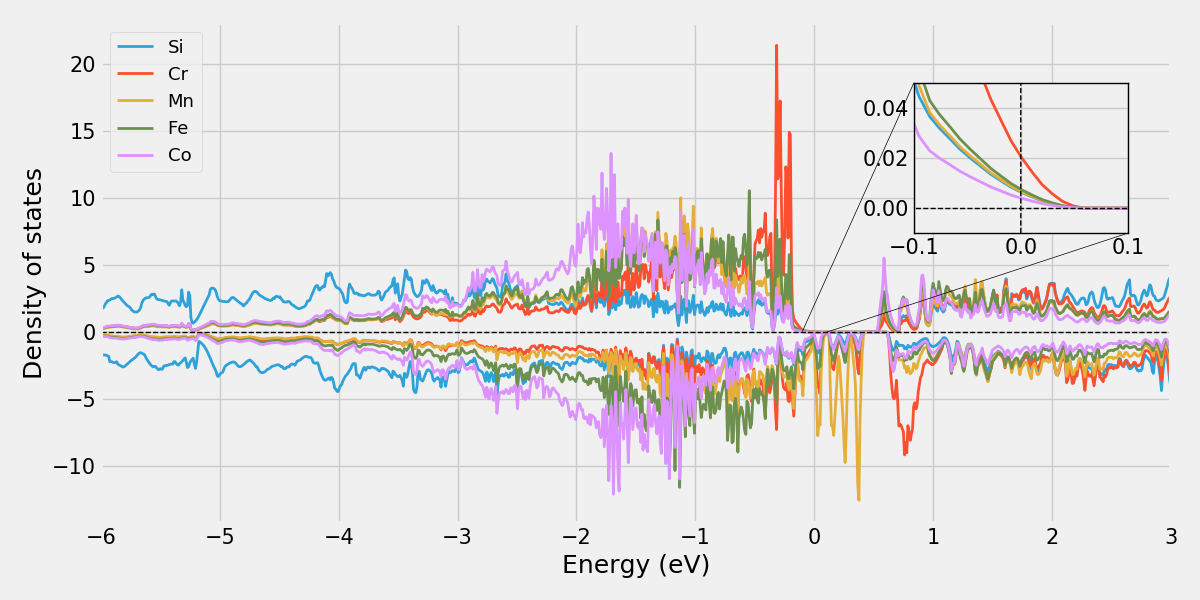
\includegraphics[width=\textwidth]{results/fesi2/composistions/crfemnco_PDOS.png}
\caption{Projected density of states of \ch{(CrFeMnCo)Si2}.}
\end{figure}

Contrary to the above case, inserting Co in the place of manganese clearly result in a metallic structure, as seen in the density of states in figure 9.2 a. Replacing Mn with Ti instead we recall from table 9.3 a a very small defect band gap in spin up, however from figure 9.2b we observe that $E_\text{G}^{dos}$ is equal to zero, thus $E_G ^\text{dos} \neq E_G ^{eigen}$. Comparing the density of states of \ch{(CrFeCoNi)Si2} and \ch{(CrFeTiNi)Si2} tha the latter is magnetic and the former nonmagnetic, as we discussed previously.  


\begin{figure}[H]
\begin{subfigure}{.5\textwidth}
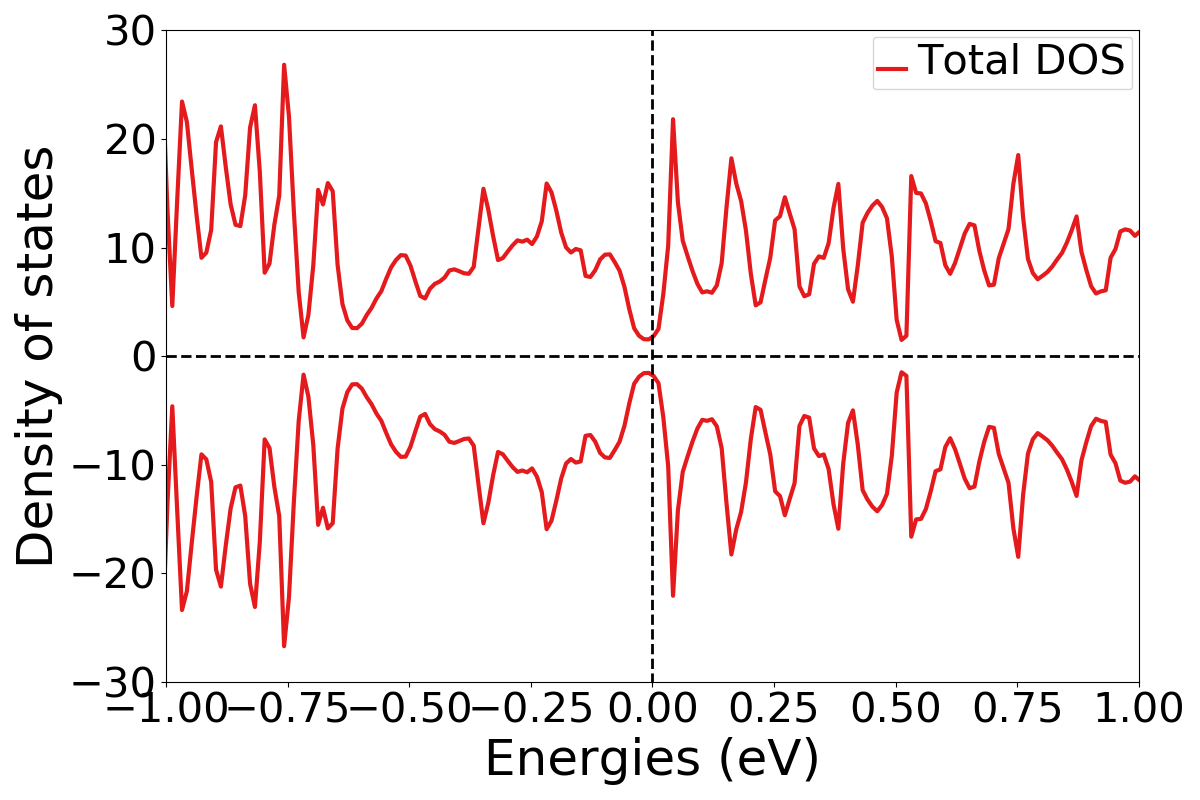
\includegraphics[width=\textwidth]{results/fesi2/composistions/crfeconi_DOS.png}
\caption{\ch{(CrFeCoNi)Si2}}
\end{subfigure}
\begin{subfigure}{.5\textwidth}
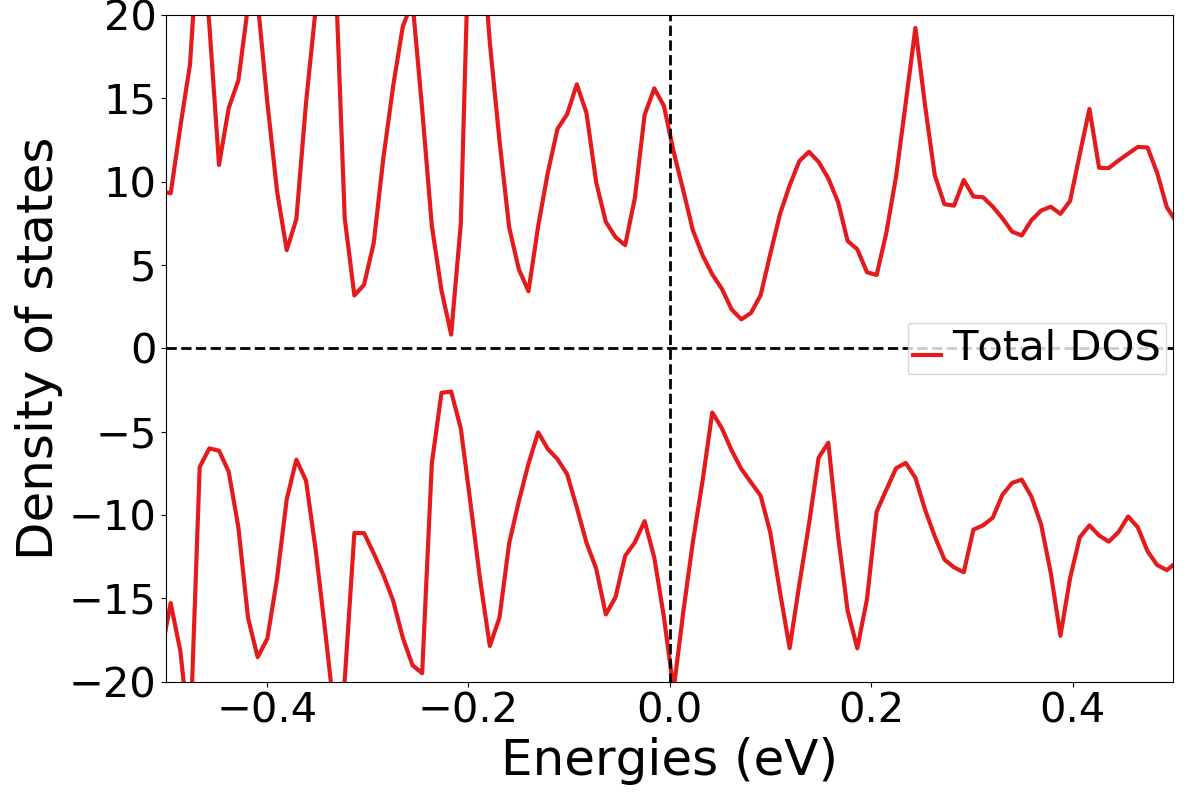
\includegraphics[width=\textwidth]{results/fesi2/composistions/crfetini_DOS.png}
\caption{\ch{(CrFeTiNi)Si2}}
\end{subfigure}
\caption{Density of states of a) \ch{(CrFeCoNi)Si2} and b) \ch{(CrFeTiNi)Si2}.}
\end{figure} 

Above we have looked at the band gap of the most stable SQS of each composition, but as we have experienced in other cases in this project, the properties can vary between SQSs of the same composition. In both \ch{CrFeCoNiSi2} and \ch{CrFeMnTiSi2} we found only metalic supercells with the exception of one SQS in the latter with a very small defect band gap in spin up. Similarly small defect band gaps was observed in two SQSs of \ch{CrFeTiNiSi2} and the rest as metals. In \ch{CrFeMnCoSi2} we found a large defect band gap in spin in the most stable configuration, here we find similar band gaps in two other SQSs as well, and two structures. The most interesting case was found in \ch{CoFeMnNiSi2} where we observed small total band gaps without defect states in two SQSs, these are seen in figure 9.3. In agreement with the nonmagnetic character of this composition, the DOS is symmetric with respect to spins. 

\begin{figure}[H]
\begin{subfigure}{.5\textwidth}
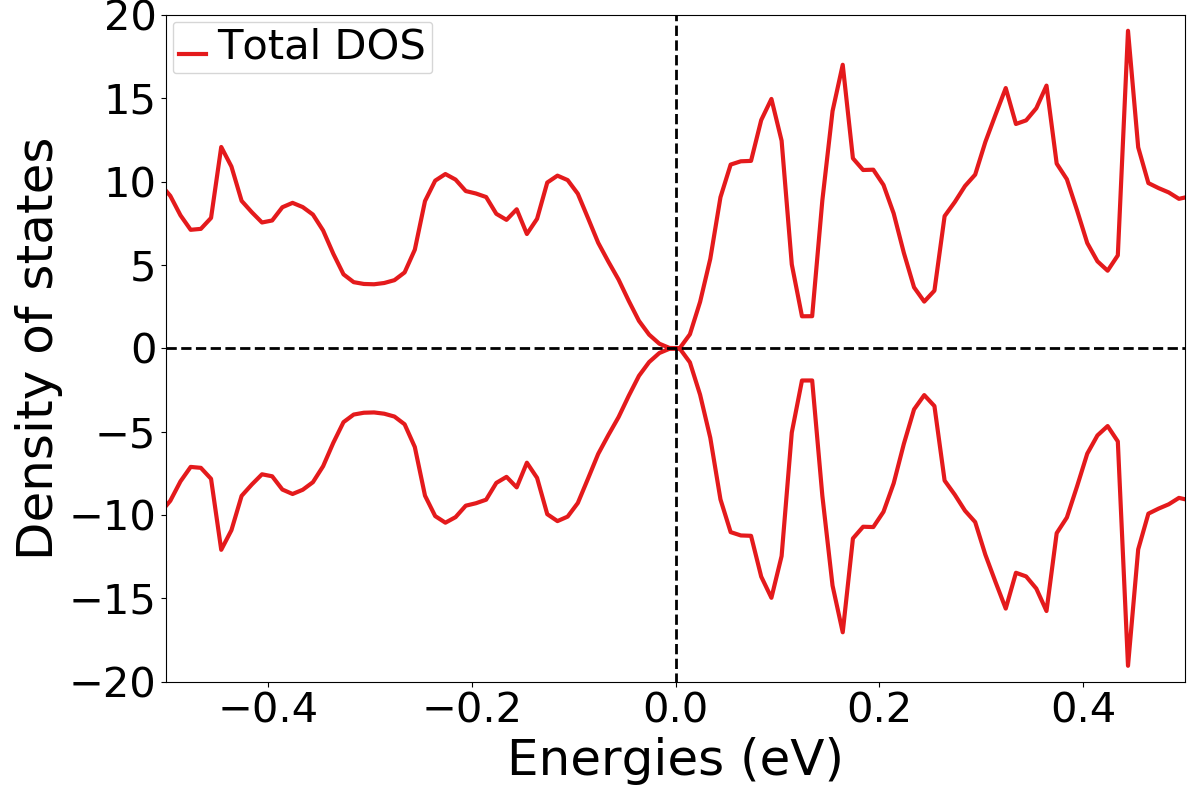
\includegraphics[width=\textwidth]{results/fesi2/composistions/cofemnni_E_DOS.png}
\caption{SQS 1}
\end{subfigure}
\begin{subfigure}{.5\textwidth}
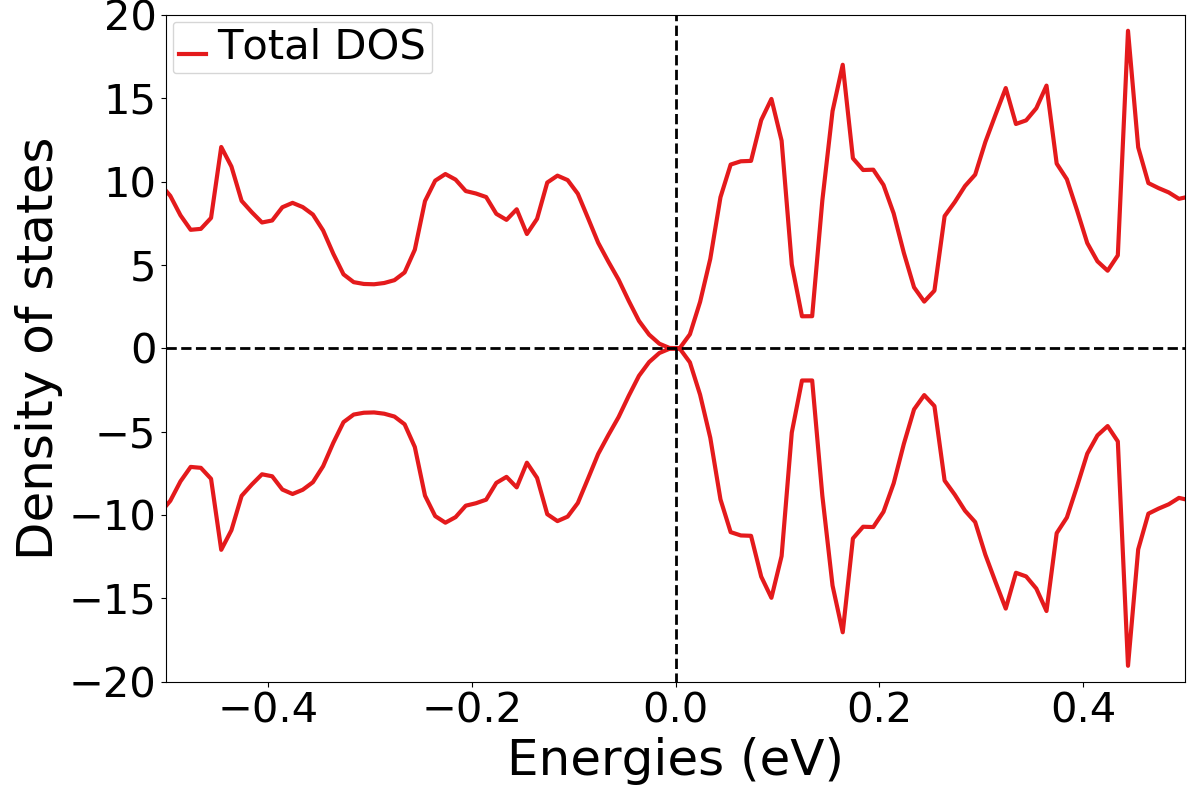
\includegraphics[width=\textwidth]{results/fesi2/composistions/cofemnni_E_DOS.png}
\caption{SQS 2}
\end{subfigure}
\caption{Density of states of two SQSs of \ch{(CoFeMnNi)Si2}.}
\end{figure} 

Thus we find examples where the most stable SQS is representative of the set, and other cases where we observe meaningful distinctions between the most stable and other possible configurations. Because of limited time examining properties and options affecting both the magnetism and stability of the alloys and respective supercells, it's important to consider the different configurations as a a broader search would not necessarily yield the same relationship. And to show some of the limitations that apply when using the special quasi-random structures method. \textbf{Can I say this?}. It appears that we find limited success overall, but particularly when substituting either Cr or Mn as outlined in the previous section. Furthermore Ti is not as successful as Co. \textbf{Continue conclusion this and entire project}
 

 